\documentclass[12pt,border=4pt,multi]{article}%\documentclass[tikz,border=4pt,multi]{article}
\usepackage{lingmacros}
\usepackage{tree-dvips}
\usepackage{amssymb} %for mathbb{}
\usepackage[dvipsnames]{xcolor}
\usepackage{forest}
\usepackage{amsmath} %for matrices
\usepackage{xeCJK}
\usepackage{tikz}
\usepackage[arrowdel]{physics}
\usepackage{graphicx}
\usepackage{wrapfig}
\usepackage{listings}
\usepackage{pgfplots, pgfplotstable}
\graphicspath{{./img}} %specify the graphics path to be relative to the main .tex file, denoting the main .tex file directory as ./
\newcommand\Myperm[2][^n]{\prescript{#1\mkern-2.5mu}{}P_{#2}}
\newcommand\Mycomb[2][^n]{\prescript{#1\mkern-0.5mu}{}C_{#2}}
\definecolor{orchid}{rgb}{0.7, 0.4, 1.1}

\begin{document}

\section*{Xi Liu, xl3504, Homework 3}
Problem 1\\
1.\\
let $\Omega$ be the sample space
\[\Omega = \{1,\; 2,\; 3,\; 4,\; 5,\; 6,\; 7,\; 8,\; 9,\; 10,\; 11,\; 12\}\]
\[A = \{2,\; 4,\; 6,\; 8,\; 10,\; 12\}\]
\[B = \{3,\; 6,\; 9,\; 12\}\]
\[A \cap B = \{6,\; 12\}\]
\[P(A) = \frac{|A|}{|\Omega|} = \frac{6}{12} = \frac{1}{2}\]
\[P(B) = \frac{|B|}{|\Omega|} = \frac{4}{12} = \frac{1}{3}\]
\[P(A \cap B) = \frac{|A \cap B|}{|\Omega|} = \frac{2}{12} = \frac{1}{6}\]
\[P(A)P(B) = \frac{1}{2}\cdot\frac{1}{3} = \frac{1}{6}\]
since 
\[P(A \cap B) = \frac{1}{6} = P(A)P(B)\]
so $A$ and $B$ are independent events for the case for which the urn contains 12 balls\\
\\
\\
\\
2.\\
\[\Omega = \{1,\; 2,\; 3,\; 4,\; 5,\; 6,\; 7,\; 8,\; 9,\; 10,\; 11,\; 12,\; 13\}\]
\[A = \{2,\; 4,\; 6,\; 8,\; 10,\; 12\}\]
\[B = \{3,\; 6,\; 9,\; 12\}\]
\[A \cap B = \{6,\; 12\}\]
\[P(A) = \frac{|A|}{|\Omega|} = \frac{6}{13}\]
\[P(B) = \frac{|B|}{|\Omega|} = \frac{4}{13}\]
\[P(A \cap B) = \frac{|A \cap B|}{|\Omega|} = \frac{2}{13}\]
\[P(A)P(B) = \frac{6}{13}\cdot\frac{4}{13} = \frac{24}{169}\]
since 
\[P(A \cap B) = \frac{2}{13} \not= \frac{24}{169} = P(A)P(B)\]
so $A$ and $B$ are not independent events for the case for which the urn contains 13 balls\\
\newpage
\noindent
Problem 2\\
let $A$ be the event that a tree in the forest has a disease\\
let $B_1$ be the event that a tree in the forest is a maple tree\\
let $B_2$ be the event that a tree in the forest is a oak tree\\
let $B_3$ be the event that a tree in the forest is a birch tree\\
\[P(B_1) = 0.3\]
\[P(B_2) = 0.5\]
\[P(B_3) = 0.2\]
\[P(A | B_1) = 0.1\]
\[P(A | B_2) = 0.04\]
\[P(A | B_3) = 0.25\]
\begin{align*}
    P(A) &= \sum_{j = 1}^3 P(A | B_j)P(B_j)\\
    &= P(A | B_1)P(B_1) + P(A | B_2)P(B_2) + P(A | B_3)P(B_3)\\
    &= (0.1)(0.3) + (0.04)(0.5) + (0.25)(0.2)\\
    &= 0.03 + 0.02 + 0.05\\
    &= 0.1\\
\end{align*}
\[P(B_1 | A) = \frac{P(B_1 \cap A)}{P(A)} = \frac{P(A | B_1)P(B_1)}{P(A)} = \frac{(0.1)(0.3)}{0.1} = \boxed{0.3}\]
\[P(B_2 | A) = \frac{P(B_2 \cap A)}{P(A)} = \frac{P(A | B_2)P(B_2)}{P(A)} = \frac{(0.04)(0.5)}{0.1} = \boxed{0.2}\]
\[P(B_3 | A) = \frac{P(B_3 \cap A)}{P(A)} = \frac{P(A | B_3)P(B_3)}{P(A)} = \frac{(0.25)(0.2)}{0.1} = \boxed{0.5}\]
verify:
\[0.3 + 0.2 + 0.5 = 1\]
\newpage
\noindent
Problem 3\\
part 1
\[P(A_i) = p_i\]
\[P(A_i^C) = 1 - p_i\]
\begin{align*}
    P(A_1 \cup A_2 \cup ... \cup A_n) &= P\left(\bigcup_{i = 1}^n A_i\right)\\
    &= 1 - P(A_1^C \cap A_2^C \cap ... \cap A_n^C)\\
    &= 1 - P\left(\bigcap_{i = 1}^n A_i^C\right)\\
    &= 1 - P(A_1^C)P(A_2^C)...P(A_n^C)\\
    &= 1 - \prod_{i = 1}^n P(A_i)^C\\
    &= 1 - (1 - p_1)(1 - p_2)...(1 - p_n)\\
    &= \boxed{1 - \prod_{i = 1}^n (1 - p_i)}\\
\end{align*}
part 2
\[P(failure) = p_i = p\]
\[P(success) = 1 - P(failure) = 1 - p\]
\begin{align*}
    P(\text{at least 1 } failure) &= 1 - \prod_{i = 1}^n (1 - p_i)\\
    &= 1 - \prod_{i = 1}^n (1 - p)\\
    &= 1 - P(success)^n\\
    &= \boxed{1 - (1 - p)^n}\\
\end{align*}
\newpage 
\noindent
Problem 4\\
for $i \in \{0,\; 1,\; 2,\; 3\}$\\
$P(X = i)$ = (number of ways to choose 2 positions that have $i$ people in between)(number of ways to arrange you and a friend)(number of ways to arrange 3 remaining people) / (number of ways to arrange 5 people)\\
\begin{align*}
P(X = 0) &= \frac{4 \cdot 2! \cdot 3!}{5!} = \boxed{\frac{4}{10}} = \frac{2}{5}\\
P(X = 1) &= \frac{3 \cdot 2! \cdot 3!}{5!} = \boxed{\frac{3}{10}}\\
P(X = 2) &= \frac{2 \cdot 2! \cdot 3!}{5!} = \boxed{\frac{2}{10}} = \frac{1}{5}\\
P(X = 3) &= \frac{1 \cdot 2! \cdot 3!}{5!} = \boxed{\frac{1}{10}}\\
\end{align*}
verify:
\[\frac{4}{10} + \frac{3}{10} + \frac{2}{10} + \frac{1}{10} = 1\]
\begin{center}
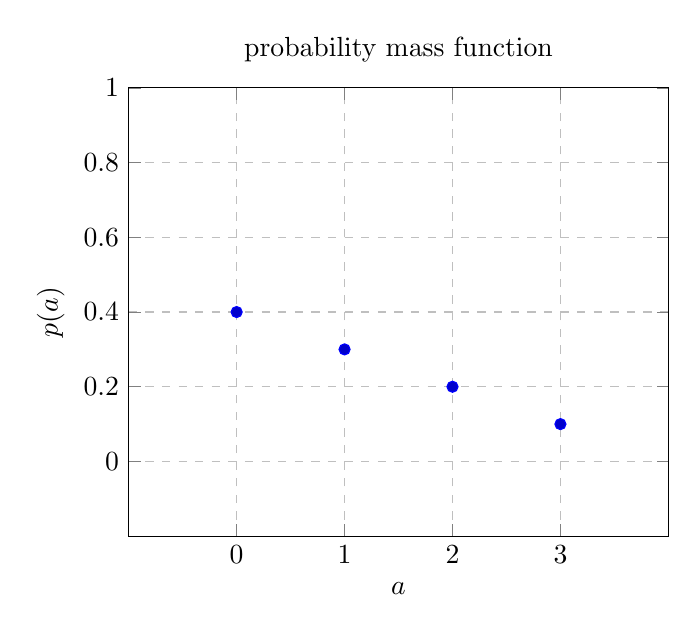
\begin{tikzpicture}
\begin{axis}[
    title={probability mass function},
    xlabel={$a$},
    ylabel={$p(a)$},
    xmin=-1, xmax=4,
    ymin=-0.2, ymax=1,
    xtick={0, 1, 2, 3},
    ytick={0, 0.2, 0.4, 0.6, 0.8, 1},
    xmajorgrids=true,
    ymajorgrids=true,
    grid style=dashed,
]
\addplot+ [only marks]
coordinates
{   
    (0, 4/10)
    (1, 3/10)
    (2, 2/10)
    (3, 1/10)
};
\end{axis}
\end{tikzpicture}
\end{center}
\begin{center}
\begin{tikzpicture}
\begin{axis}
[
    title={cumulative distribution function},
    xlabel={$a$},
    ylabel={$F(a)$},
    jump mark left,
    xmin=-1, xmax=4,
    ymin=-0.2, ymax=1.2,
    xtick={0, 1, 2, 3},
    ytick={0, 4/10, 7/10, 9/10, 1},
    every axis plot/.style={very thick},
    discontinuous,
    xmajorgrids=true,
    ymajorgrids=true,
    grid style=dashed,
    table/create on use/cumulative distribution/.style={
        create col/expr={\pgfmathaccuma + \thisrow{f(x)}}   
    }
]
\addplot table [y=cumulative distribution]
{
    x f(x)
    -2 0
    0 4/10
    1 3/10
    2 2/10
    3 1/10
    5 0
};
\end{axis}
\end{tikzpicture}
\end{center}
\newpage
\noindent
Problem 5\\
let $D$ be the outcome that the inspector selects a defective hard drive\\
let $N$ be the outcome that the inspector selects a not defective hard drive\\
\\
$X = 0$ is when the inspector selects 3 not defective hard drives, $\{NNN\}$
\[P(X = 0) = \frac{34}{40}\cdot\frac{33}{39}\cdot\frac{32}{38} = \binom{3}{0}\cdot\frac{34}{40}\cdot\frac{33}{39}\cdot\frac{32}{38} = \boxed{\frac{748}{1235}}\]
$X = 1$ is when the inspector selects 1 defective hard drive and 2 not defective hard drives, $\{DNN,\;NDN,\;NND\}$
\begin{align*}
P(X = 1) &= \frac{6}{40}\cdot\frac{34}{39}\cdot\frac{33}{38} + \frac{34}{40}\cdot\frac{6}{39}\cdot\frac{33}{38} + \frac{34}{40}\cdot\frac{33}{39}\cdot\frac{6}{38}\\
&= \binom{3}{1}\cdot\frac{6}{40}\cdot\frac{34}{39}\cdot\frac{33}{38} = \boxed{\frac{1683}{4940}}\\
\end{align*}
$X = 2$ is when the inspector selects 2 defective hard drive and 1 not defective hard drives,
$\{DDN,\;DND,\;NDD\}$
\begin{align*}
P(X = 2) &= \frac{6}{40}\cdot\frac{5}{39}\cdot\frac{34}{38} + \frac{6}{40}\cdot\frac{34}{39}\cdot\frac{5}{38} + \frac{34}{40}\cdot\frac{6}{39}\cdot\frac{5}{38}\\
&= \binom{3}{2}\cdot\frac{6}{40}\cdot\frac{5}{39}\cdot\frac{34}{38} = \boxed{\frac{51}{988}}\\   
\end{align*}
$X = 3$ is when the inspector selects 3 defective hard drives, $\{DDD\}$
\begin{align*}
P(X = 3) = \frac{6}{40}\cdot\frac{5}{39}\cdot\frac{4}{38} = \binom{3}{3}\cdot\frac{6}{40}\cdot\frac{5}{39}\cdot\frac{4}{38} = \boxed{\frac{1}{494}}
\end{align*}
verify:
\[\frac{748}{1235} + \frac{1683}{4940} + \frac{51}{988} + \frac{1}{494} = 1\]
\begin{center}
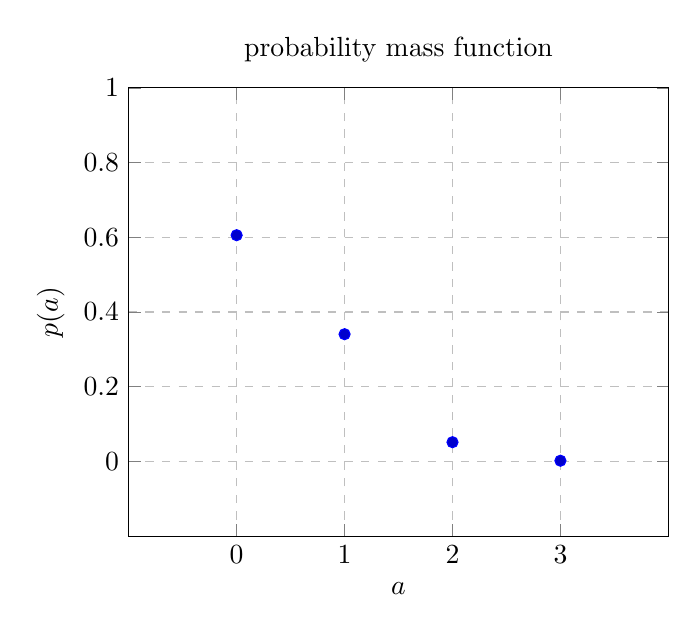
\begin{tikzpicture}
\begin{axis}[
    title={probability mass function},
    xlabel={$a$},
    ylabel={$p(a)$},
    xmin=-1, xmax=4,
    ymin=-0.2, ymax=1,
    xtick={0, 1, 2, 3},
    ytick={0, 0.2, 0.4, 0.6, 0.8, 1},
    xmajorgrids=true,
    ymajorgrids=true,
    grid style=dashed,
]
\addplot+ [only marks]
coordinates
{   
    (0, 748/1235)
    (1, 1683/4940)
    (2, 51/988)
    (3, 1/494)
};
\end{axis}
\end{tikzpicture}
\end{center}
\begin{center}
\begin{tikzpicture}
\begin{axis}
[
    title={cumulative distribution function},
    xlabel={$a$},
    ylabel={$F(a)$},
    jump mark left,
    xmin=-1, xmax=4,
    ymin=-0.2, ymax=1.2,
    xtick={0, 1, 2, 3},
    ytick={0, 748/1235, 748/1235+1683/4940, 748/1235+1683/4940+51/988, 748/1235+1683/4940+51/988+1/494, 1},
    every axis plot/.style={very thick},
    discontinuous,
    xmajorgrids=true,
    ymajorgrids=true,
    grid style=dashed,
    table/create on use/cumulative distribution/.style={
        create col/expr={\pgfmathaccuma + \thisrow{f(x)}}   
    }
]
\addplot table [y=cumulative distribution]
{
    x f(x)
    -2 0
    0 748/1235
    1 1683/4940
    2 51/988
    3 1/494
    5 0
};
\end{axis}
\end{tikzpicture}
\end{center}
\end{document}